%%%%%%%%%%%%%%%%%%%%%%%%%%%%%%%%%%%%%%%%%%%%%%%%%%%%%%%%%%%%%%%%%%%%%%
%%  Copyright by Wenliang Du.                                       %%
%%  This work is licensed under the Creative Commons                %%
%%  Attribution-NonCommercial-ShareAlike 4.0 International License. %%
%%  To view a copy of this license, visit                           %%
%%  http://creativecommons.org/licenses/by-nc-sa/4.0/.              %%
%%%%%%%%%%%%%%%%%%%%%%%%%%%%%%%%%%%%%%%%%%%%%%%%%%%%%%%%%%%%%%%%%%%%%%

\documentclass[11pt]{article}

\usepackage[most]{tcolorbox}
\usepackage{times}
\usepackage{epsf}
\usepackage{epsfig}
\usepackage{amsmath, alltt, amssymb, xspace}
\usepackage{wrapfig}
\usepackage{fancyhdr}
\usepackage{url}
\usepackage{verbatim}
\usepackage{fancyvrb}
\usepackage{adjustbox}
\usepackage{listings}
\usepackage{color}
\usepackage{subfigure}
\usepackage{cite}
\usepackage{sidecap}
\usepackage{pifont}
\usepackage{mdframed}
\usepackage{textcomp}
\usepackage{enumitem}
\usepackage{ctex}


% Horizontal alignment
\topmargin      -0.50in  % distance to headers
\oddsidemargin  0.0in
\evensidemargin 0.0in
\textwidth      6.5in
\textheight     8.9in 

\newcommand{\todo}[1]{
\vspace{0.1in}
\fbox{\parbox{6in}{TODO: #1}}
\vspace{0.1in}
}


\newcommand{\unix}{{\tt Unix}\xspace}
\newcommand{\linux}{{\tt Linux}\xspace}
\newcommand{\minix}{{\tt Minix}\xspace}
\newcommand{\ubuntu}{{\tt Ubuntu}\xspace}
\newcommand{\setuid}{{\tt Set-UID}\xspace}
\newcommand{\openssl} {\texttt{openssl}}


\pagestyle{fancy}
\lhead{\bfseries SEED Labs}
\chead{}
\rhead{\small \thepage}
\lfoot{}
\cfoot{}
\rfoot{}


\definecolor{dkgreen}{rgb}{0,0.6,0}
\definecolor{gray}{rgb}{0.5,0.5,0.5}
\definecolor{mauve}{rgb}{0.58,0,0.82}
\definecolor{lightgray}{gray}{0.90}


\lstset{%
  frame=none,
  language=,
  backgroundcolor=\color{lightgray},
  aboveskip=3mm,
  belowskip=3mm,
  showstringspaces=false,
%  columns=flexible,
  basicstyle={\small\ttfamily},
  numbers=none,
  numberstyle=\tiny\color{gray},
  keywordstyle=\color{blue},
  commentstyle=\color{dkgreen},
  stringstyle=\color{mauve},
  breaklines=true,
  breakatwhitespace=true,
  tabsize=3,
  columns=fullflexible,
  keepspaces=true,
  escapeinside={(*@}{@*)}
}

\newcommand{\newnote}[1]{
\vspace{0.1in}
\noindent
\fbox{\parbox{1.0\textwidth}{\textbf{Note:} #1}}
%\vspace{0.1in}
}


%% Submission
\newcommand{\seedsubmission}{You need to submit a detailed lab report, with screenshots,
to describe what you have done and what you have observed.
You also need to provide explanation
to the observations that are interesting or surprising.
Please also list the important code snippets followed by
explanation. Simply attaching code without any explanation will not
receive credits.}

%% Book
\newcommand{\seedbook}{\textit{Computer \& Internet Security: A Hands-on Approach}, 2nd
Edition, by Wenliang Du. See details at \url{https://www.handsonsecurity.net}.}

%% Videos
\newcommand{\seedisvideo}{\textit{Internet Security: A Hands-on Approach},
by Wenliang Du. See details at \url{https://www.handsonsecurity.net/video.html}.}

\newcommand{\seedcsvideo}{\textit{Computer Security: A Hands-on Approach},
by Wenliang Du. See details at \url{https://www.handsonsecurity.net/video.html}.}

%% Lab Environment
\newcommand{\seedenvironment}{This lab has been tested on our pre-built
Ubuntu 16.04 VM, which can be downloaded from the SEED website.}






\newcommand{\seedlabcopyright}[1]{
\vspace{0.1in}
\fbox{\parbox{6in}{\small Copyright \copyright\ {#1}\ \ by Wenliang Du.\\
      This work is licensed under a Creative Commons
      Attribution-NonCommercial-ShareAlike 4.0 International License.
      If you remix, transform, or build upon the material, 
      this copyright notice must be left intact, or reproduced in a way that is reasonable to
      the medium in which the work is being re-published.}}
\vspace{0.1in}
}






\newcommand{\pkiFigs}{./Figs}

\newcommand{\OpenSSL} {\texttt{OpenSSL}\xspace}
\newcommand{\pkiserver}{\texttt{SEEDPKILab2020.com}\xspace}

\lhead{\bfseries SEED Labs -- PKI 实验}


\begin{document}

\begin{center}
{\LARGE 公钥基础设施 (PKI) 实验}
\end{center}

\seedlabcopyright{2018}



% *******************************************
% SECTION
% *******************************************
\section{概述}



公钥密码学是当今安全通信的基础。
但是当通信的一方将其公钥发送给另一方时,会受到中间人的攻击。
根本的问题是,验证公钥的所有权不是一个容易解决的问题。
也就是给定公钥及其声明的所有者信息,我们如何确保公钥确实由声明的所有者拥有?
公钥基础设施(PKI)就是解决此问题的一种方法。


该实验的目的是让学生获得有关PKI的第一手经验。
SEED labs 有一系列关于公钥加密的实验,而这个实验则针对PKI。
通过完成本实验中的任务,学生应该能够更好地理解PKI的工作原理,了解如何使用PKI保护Web以及如何用PKI克服中间人攻击。
此外,学生将能够了解公钥基础设施中信任的根源,以及如果信任根被破坏,将会出现哪些问题。
本实验涵盖以下主题:

\begin{itemize}[noitemsep]
\item 公钥加密
\item 公钥基础设施(PKI)
\item 证书颁发机构(CA)和根 CA
\item X.509 证书和自签名证书
\item Apache, HTTP, 和 HTTPS
\item 中间人攻击
\end{itemize}



\paragraph{阅读材料}
有关PKI的详细信息,请阅读以下内容:

\begin{itemize}
\item Chapter 23 of the SEED Book, \seedbook
\end{itemize}


\paragraph{相关实验}

与本实验相关的一个话题是基于PKI的传输层安全(TLS)。我们有一个单独的TLS实验。
另外,还有一个 \textit{RSA公钥加密和签名实验},其重点是公钥加密的算法部分。


\paragraph{实验环境} \seedenvironment



% *******************************************
% SECTION
% *******************************************
\section{实验内容}


% -------------------------------------------
% SUBSECTION
% -------------------------------------------
\subsection{任务 1: 构建一个证书颁发机构(CA)}

证书颁发机构(CA)是颁发数字证书的一个受信任的实体。
数字证书通过证书指定的主体(Subject)证明公钥的所有权。
有许多商业化的CA被视为根CA。
在撰写本文时,VeriSign是最大的CA。
用户需要付费才能获得这些商业CA颁发的数字证书。


在这个实验中,我们需要创建数字证书,但是我们不会向任何商业CA付费。
我们会自己创建一个根CA,然后使用该CA为其他实体(例如服务器)颁发证书。
在此任务中,我们将自己设为根CA,并为此CA生成一个证书。
与通常由另一个CA签名的其他证书不同,根CA的证书是自签名的。
根CA的证书通常预加载到大多数操作系统,Web浏览器和其他依赖PKI的软件中。
根CA的证书是无条件信任的。


\paragraph{配置文件 {\tt openssl.conf}}
要使用 \OpenSSL 来创建证书,首先需要有一个配置文件。
配置文件的扩展名通常为 {\tt .cnf}。
在 \OpenSSL 的 {\tt ca}、 {\tt req} 和 {\tt x509} 命令中会使用到这个配置文件。
\texttt{openssl.conf} 的说明文档可以用搜索引擎找到,
也可以在 \path{/usr/lib/ssl/openssl.cnf} 中找到一份配置文件。
把这个文件复制到你的当前目录之后,你需要创建几个在配置文件中指定的子目录
(参阅 {\tt [CA\_default]} 一节):


\begin{lstlisting}
   dir             = ./demoCA        # Where everything is kept
   certs           = $dir/certs      # Where the issued certs are kept
   crl_dir         = $dir/crl        # Where the issued crl are kept
   new_certs_dir   = $dir/newcerts   # default place for new certs.
   database        = $dir/index.txt  # database index file.
   serial          = $dir/serial     # The current serial number
\end{lstlisting}

对于 \texttt{index.txt} 文件, 创建一个空文件即可。
对于 \texttt{serial} ,放一个字符串格式的数(例如 1000)在文件中。
当你设置好了配置文件 \texttt{openssl.cnf} 之后就可以创建和颁发证书了。


\paragraph{证书颁发机构(CA)}
如前所述,我们需要为我们的CA生成一个自签名证书。
这意味着该CA是完全受信任的,并且其证书将用作根证书。
你可以运行以下命令为CA生成自签名证书:

\begin{lstlisting}[backgroundcolor=]
$ openssl req -new -x509 -keyout ca.key -out ca.crt -config openssl.cnf
\end{lstlisting}

系统将提示你输入一些信息和密码。
不要丢失此密码,因为每次要使用此CA为其他人签名证书时,都必须输入密码。
它还将要求填写一些信息,例如“国家名称”,“通用名称”等。
命令的输出存储在两个文件中:{\tt ca.key} 和 {\tt ca.crt}。
文件{\tt ca.key}包含CA的私钥,而{\tt ca.crt}包含公钥证书。



% -------------------------------------------
% SUBSECTION
% -------------------------------------------
\subsection{任务 2: 为 \pkiserver 创建一个证书}

现在我们已经成为了一个根CA,准备给我们的客户签发数字证书。
我们的第一个客户是一个名为 \pkiserver 的公司。
为了使该公司从CA获得数字证书,需要经历三个步骤。

\paragraph{第 1 步: 生成公私钥对}
公司首先需要创建自己的公私钥对。
我们可以运行以下命令来生成RSA密钥对(私钥和公钥)。
你还需要提供密码来加密私钥(在命令选项指定了使用AES-128加密算法)。
密钥将存储在文件 \texttt{server.key} 中:

\begin{lstlisting}[backgroundcolor=]
$ openssl genrsa -aes128 -out server.key 1024
\end{lstlisting}

\texttt{server.key} 是一个经过编码(和加密)的文本文件,因此你无法看到实际的内容,例如模数,私有指数等。
要查看这些内容,可以运行以下命令:

\begin{lstlisting}[backgroundcolor=]
$ openssl rsa -in server.key -text
\end{lstlisting}



\paragraph{第 2 步: 生成一个证书签发请求 (CSR).}
公司拥有密钥文件后,应当生成一个证书签名请求(CSR)。
该证书签名请求会包括公司的公钥。
CSR将被发送到CA,CA将为密钥生成证书(在确保CSR中的身份信息与服务器的真实身份匹配之后)。
请使用 \pkiserver 作为证书请求的通用名称(Common Name)。

\begin{lstlisting}[backgroundcolor=]
$ openssl req -new -key server.key -out server.csr -config openssl.cnf
\end{lstlisting}


注意到,以上命令与我们在为CA创建自签名证书时使用的命令非常相似。
它们唯一的区别是{\tt -x509}选项。
没有这个选项,该命令将生成一个证书签发请求;
加上这个选项,该命令将生成一个自签名证书。

\paragraph{第 3 步: 生成证书}
CSR文件需要具有CA的签名才能形成证书。
在现实世界中,通常将CSR文件发送到受信任的CA进行签名。
在本实验中,我们将使用我们自己的受信任CA生成证书。
以下命令使用CA的 {\tt ca.crt} 和 {\tt ca.key} ,将证书签名请求( {\tt server.csr} )转换为X509证书({\tt server.crt}):

\begin{lstlisting}[backgroundcolor=]
$ openssl ca -in server.csr -out server.crt -cert ca.crt -keyfile ca.key \
             -config openssl.cnf
\end{lstlisting}

如果 \OpenSSL 拒绝生成证书,那么你的请求中的名称很可能与 CA 的名称不匹配。
匹配规则在配置文件中指定(请参见 \texttt{[policy\_match]} 部分)。
你可以更改请求名称以符合策略,也可以更改策略。
配置文件还包含另一个策略(称为 \texttt {policy\_anything}),该策略的限制较少。
你可以通过更改以下行来选择该策略:

\begin{lstlisting}[backgroundcolor=]
   "policy = policy_match"  change to "policy = policy_anything".
\end{lstlisting}



% -------------------------------------------
% SUBSECTION
% -------------------------------------------
\subsection{任务 3: 部署证书到一个 HTTPS Web 服务器上}

在本实验中,我们将探索网站是如何用证书来保护 Web 的。
我们将使用 \OpenSSL 的内置Web服务器建立一个HTTPS网站。


\paragraph{第 1 步: 配置DNS}
我们选择 {\pkiserver} 作为网站的名字.
为了让我们的计算机能识别这个名字,我们需要在 \texttt{/etc/hosts} 中添加下面这一项。
这一项把域名 {\pkiserver} 映射到 localhost (也就是 127.0.0.1):


\begin{lstlisting}[backgroundcolor=]
   127.0.0.1  SEEDPKILab2018.com
\end{lstlisting}


\paragraph{第 2 步: 配置 Web 服务器}
让我们使用上一个任务中生成的证书启动一个简单的 Web 服务器。
\OpenSSL 允许我们使用 \texttt{s\_server} 命令启动简单的 Web 服务器:

\begin{lstlisting}
  # Combine the secret key and certificate into one file
  % cp server.key server.pem
  % cat server.crt >> server.pem

  # Launch the web server using server.pem
  % openssl s_server -cert server.pem -www
\end{lstlisting}

默认情况下,服务器会监听 {\tt 4433} 端口。
你可以使用 {\tt -accept} 选项更改端口。
现在,使用以下 URL 访问服务器:\url{https://SEEDPKILab2018.com:4433/}。
你将很有可能在浏览器中看到一条错误消息。
在 Firefox 中,你会看到类似这样的消息:
{\em ``seedpkilab2018.com:4433 uses an invalid security certificate. The certificate is not trusted because the issuer certificate is unknown''.}


\paragraph{第 3 步: 使浏览器接受我们的证书}
如果我们的证书是由 VeriSign 分配的,我们将不会收到这样的错误消息,因为 VeriSign 的证书很有可能已经预先加载到 Firefox 的证书库中。
不幸的是,\pkiserver 证书是由我们自己的CA签名的(即使用 {\tt ca.crt}),并且 Firefox 无法识别该CA。
有两种方法可以使 Firefox 接受我们的CA自签名证书。

\begin{itemize}

\item 我们可以要求 Mozilla 在其 Firefox 软件中加入我们的CA证书,这样使用 Firefox 的每个人都可以识别我们的CA。
这就是真正的CA(例如VeriSign)将其证书添加到Firefox中的方式。
不幸的是,我们自己的CA没有足够大的市场供Mozilla包含我们的证书,因此我们不会采用这种方法。

\item {\bf 将 {\tt ca.crt} 导入 Firefox :}
通过点击以下菜单,我们可以将CA的证书手动添加到 Firefox 浏览器:

\begin{lstlisting}[backgroundcolor=]
   Edit -> Preference -> Privacy & Security -> View Certificates.
\end{lstlisting}

你会看到Firefox已经接受的证书列表。
从这里,我们可以 ``导入'' 我们自己的证书。
请导入 {\tt ca.crt} ,然后选择 ``信任此CA可以标识网站'' 。
你会看到我们的CA证书现在位于Firefox的已接受证书列表中。
\end{itemize}


\paragraph{第 4 步: 测试我们的 HTTPS 网站}
现在访问 \url{https://SEEDPKILab2018.com:4433}。
请描述和解释你观察到的现象,并完成以下任务:

\begin{enumerate}
\item 修改 {\tt server.pem} 中的一个字节,重新启动服务器并刷新页面。
      你观察到了什么?
      确保你之后能回复原始的 {\tt server.pem}。
      注意:如果 {\tt server.pem} 中某些特定的部分被破坏,服务器可能无法重启。
      在这种情况下,选择另一个位置修改。


\item 既然 \pkiserver 指向了 localhost,访问 \url{https://localhost:4433} 将会连接到同一个 Web 服务器。
      请这样尝试一下,描述并解释你观察到的现象。
\end{enumerate}



% -------------------------------------------
% SUBSECTION
% -------------------------------------------
\subsection{任务 4: 在基于Apache的HTTPS网站中部署证书}


使用 \openssl 的 \texttt{s\_server} 命令设置 HTTPS 服务器主要用于调试和演示。
在本实验中,我们基于 Apache 建立了一个真实的 HTTPS Web 服务器。
我们的VM中已经安装了Apache服务器,它支持HTTPS协议。
要创建HTTPS网站,我们只需要配置Apache服务器,让它知道从哪里获取私钥和证书。
我们在下面给出一个示例,演示如何为网站 \url{www.example.com} 启用HTTPS。
你的任务是使用从先前任务生成的证书对 {\pkiserver} 执行相同的操作。

一个Apache服务器可以同时托管多个网站。
它需要知道网站文件的存储目录。
这是通过位于 \url{/etc/apache2/sites-available} 目录中的 \texttt{VirtualHost} 文件完成的。
要添加HTTP网站,我们将 \texttt{VirtualHost} 条目添加到文件 \texttt{000-default.conf}。
请参见以下示例。

\begin{lstlisting}
<VirtualHost *:80>
    ServerName one.example.com
    DocumentRoot /var/www/Example_One
    DirectoryIndex index.html
</VirtualHost>
\end{lstlisting}

要添加一个 HTTPS 网站,我们需要在相同文件夹里的 \texttt{default-ssl.conf} 文件中添加一个 \texttt{VirtualHost} 条目。

\begin{lstlisting}
<VirtualHost *:443>
    ServerName two.example.com
    DocumentRoot /var/www/Example_Two
    DirectoryIndex index.html

    SSLEngine On
    SSLCertificateFile      /etc/apache2/ssl/example_cert.pem  (*@\ding{192}@*)
    SSLCertificateKeyFile   /etc/apache2/ssl/example_key.pem   (*@\ding{193}@*)
</VirtualHost>
\end{lstlisting}

\texttt{ServerName} 指明了网站的名字,而 \texttt{DocumentRoot} 指明了存放网站文件的位置。
上面的例子配置了 HTTPS 网站 \url{https://two.example.com}  (端口 \texttt{443}
是 HTTPS 的默认端口)。
在设置中,我们需要告诉 Apache 服务器证书 (\ding{192}) 和私钥 (\ding{193}) 存放在了哪里。


在 \texttt{default-ssl.conf} 文件被修改以后,我们需要运行一系列命令来启用 SSL。
Apache 将会要求我们输入用于加密私钥的密码。
当这些都正确和之后以后,我们可以浏览这个网站。
浏览器与服务器之间所有的流量都会被加密。

\begin{lstlisting}
 // Test the Apache configuration file for errors
 $ sudo apachectl configtest

 // Enable the SSL module
 $ sudo a2enmod ssl

 // Enable the site we have just edited
 $ sudo a2ensite default-ssl

 // Restart Apache
 $ sudo service apache2 restart
\end{lstlisting}



请使用参考以上示例为 \pkiserver 设置 HTTPS 服务器。
请描述你的操作步骤,添加到 Apache 的配置文件中的内容以及最终结果的屏幕截图,以展示你可以成功浏览HTTPS站点。



% -------------------------------------------
% SUBSECTION
% -------------------------------------------
\subsection{任务 5: 发起中间人攻击}

在此任务中,我们将展示 PKI 如何抵御中间人(MITM)攻击。
图 \ref{pki:fig:mitm} 描述了MITM攻击的工作方式。
假设 Alice 想通过HTTPS协议访问 \texttt{example.com}。
她需要从 \texttt{example.com} 服务器获取公钥; Alice 将生成一个秘密,并使用服务器的公钥对该秘密进行加密,然后将其发送到服务器。
如果攻击者可以拦截 Alice 与服务器之间的通信,那么攻击者可以用其自己的公钥替换服务器的公钥。
这样 Alice 的秘密实际上是使用攻击者的公钥加密的,因此攻击者将能够读取该秘密。
攻击者可以使用服务器的公钥将秘密转发给服务器。
因为该秘密将用于加密 Alice 和服务器之间的通信,因此攻击者可以解密加密的通信。


\begin{figure}[htb]
   \begin{center}
      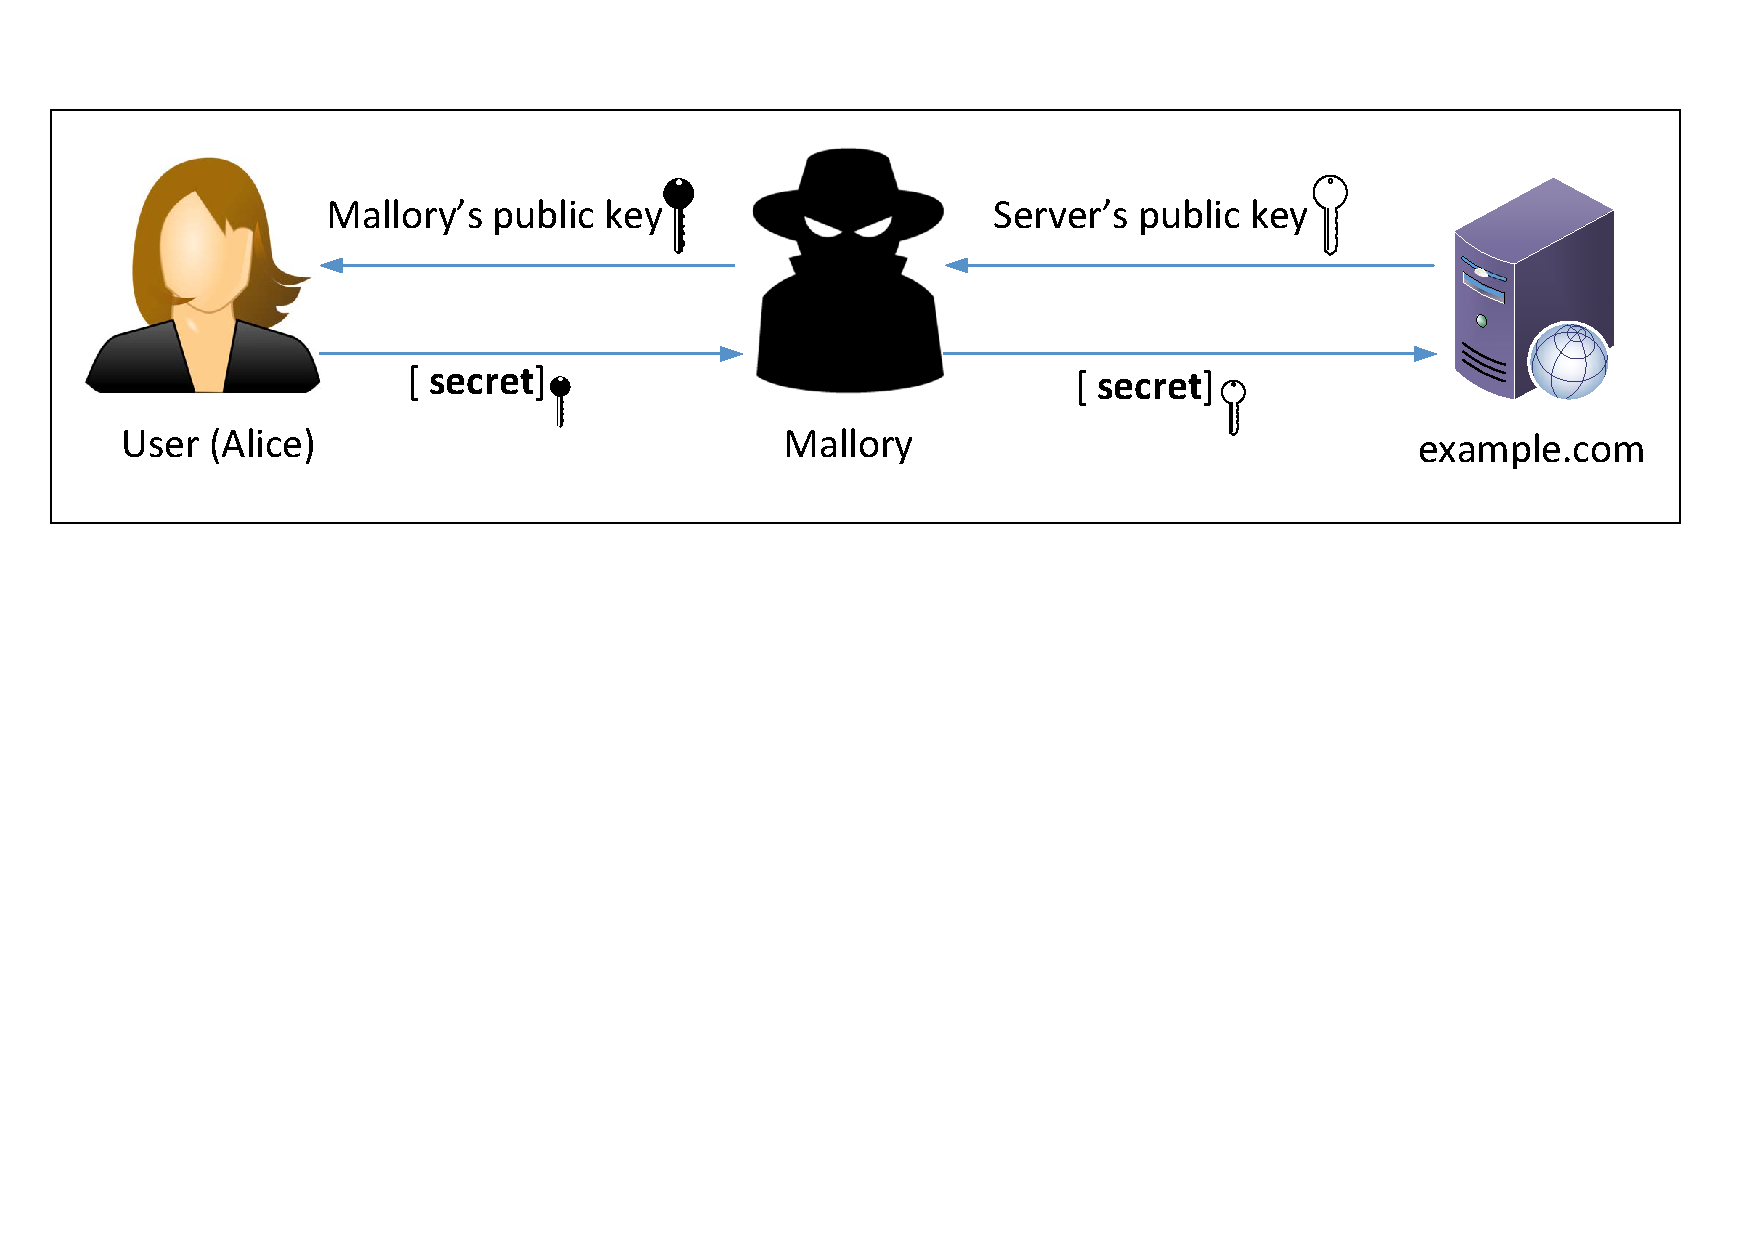
\includegraphics[width=0.8\textwidth]{\pkiFigs/mitm.pdf}
   \end{center}
   \caption{中间人攻击}
   \label{pki:fig:mitm}
\end{figure}



该任务的目的是帮助学生了解 PKI 如何抵御此类MITM攻击。
在任务中,我们将模拟一次MITM攻击,并了解PKI如何精确地防御。
我们将首先选择一个目标网站。
在本文档中,我们使用 \texttt{example.com} 作为目标网站。
但在实际任务中,为了使其更有意义,学生可以选择一个受欢迎的网站,例如银行网站或者社交网站。


\paragraph{第 1 步: 启动一个恶意网站}
在任务4中,我们已经为 \pkiserver 建立了HTTPS网站。
我们将使用同一台 Apache 服务器来模拟 \texttt{example.com} (或学生选择的站点)。
为此,我们将按照任务4中的说明向Apache的SSL配置文件中添加 \texttt{VirtualHost} 条目, \texttt{ServerName} 应该为 \texttt{example.com} ,但其余配置可以与任务4中使用的相同。
我们的目标如下:当用户尝试访问 \texttt{example.com} 时,我们将使该用户进入我们的服务器,该服务器托管一个伪造的 \texttt{example.com}。
如果这是一个社交网络网站,则假网站可以显示类似于目标网站中的登录页面。
如果用户无法分辨出区别,则可以在伪造的网页中键入其帐户凭据,从而使攻击者获得凭据。


\paragraph{第 2 步: 成为中间人}
有几种方法可以使用户的 HTTPS 请求进入我们的 Web 服务器。
一种方法是路由攻击,使用户的 HTTPS 请求被路由到我们的 Web 服务器。
另一种方法是 DNS 攻击,当受害者的计算机尝试找出目标 Web 服务器的 IP 地址时,它将获取我们 Web 服务器的 IP 地址。
在此任务中,我们使用 DNS 攻击。 无需发动实际的 DNS 缓存中毒攻击,我们只需修改受害者机器的 \texttt{/etc/hosts} 文件,以模拟 DNS 缓存存储攻击的结果(应使用恶意服务器的实际IP地址替换 \texttt{IP\_Address})。



\begin{lstlisting}[backgroundcolor=]
   <IP_Address>  example.com
\end{lstlisting}


\paragraph{第 3 步: 浏览目标网站}
完成所有设置后,现在访问目标真实网站,并查看您的浏览器会说些什么。
请解释你观察到的现象。




% -------------------------------------------
% SUBSECTION
% -------------------------------------------
\subsection{任务 6: 使用一个被攻陷的 CA 发起中间人攻击}

不幸的是,我们在任务1中创建的根CA被攻击者攻破,并且其私钥被盗。
因此,攻击者可以使用此CA的私钥生成任意证书。
在此任务中,我们将看到这种破坏的结果。



请设计一个实验,以表明攻击者可以在任何HTTPS网站上成功发起MITM攻击。
你可以使用在任务5中创建的相同设置,但是这次,你需要证明MITM攻击是成功的。
即当受害人试图访问网站时,浏览器不会有起任何怀疑,而是落入MITM攻击者的虚假网站。




% *******************************************
% SECTION
% *******************************************
\section{提交}

\seedsubmission


%%%%%%%%%%%%%%%%%%%%%%%%%%%%%%%%%%%%%%%%%%%%%%%%%%%%%%
\end{document}
%%%%%%%%%%%%%%%%%%%%%%%%%%%%%%%%%%%%%%%%%%%%%%%%%%%%%%

